\documentclass[aspectratio=169]{beamer}

\usepackage{mystyle}

\title{Measuring the Information Content of VIX Volatility}
\author{Context: Humboldt Project\\
Supervisor: Prof. Franziska Peter\\
Author: Sophia Gläser (7. Semester BA CME)}
\date{\small \today}

\addbibresource{./bib/bibliography.bib} 

\begin{document}

\begin{frame}
\maketitle
\end{frame}

\begin{frame}
\frametitle{Table of Contents}
\tableofcontents
\end{frame}

\section{Introduction}

\begin{frame}
\frametitle{Motivation: Why this project? Why does Volatility matter?}
	\begin{itemize}
	\item<1-> For the stability of the financial system, precise risk measurement is of great importance
	\begin{itemize}
	\item<1-> Volatility is closely related to risk 
	\item<1-> it is crucial input to risk measures, such as the Value at Risk\footnote{The Value at Risk is a quantile of the loss function, used for example by banks to estimate the amount of assets needed to cover possible losses. It estimates which loss is not going to be exceeded in a given time interval, for a given probability}
	\end{itemize}
	\item<2-> Moreover volatility is used for..
	\begin{itemize}
	\item<2-> .. the pricing of financial instruments, such as derivatives
	\item<2-> .. the risk-return trade-off and therefore management decisions
	\end{itemize}
	\end{itemize}
\end{frame}

\begin{frame}
\frametitle{More closely: What exactly is Volatility?}
	\begin{itemize}
	\item<1-> In Finance, we are usually interested in the \textit{conditional} standard deviation from the expected value of the underlying asset return \parencite{tsay2005}
	\item<1-> What causes asset price movement and thus volatility?
	\begin{itemize}
	\item<2-> Assuming Market efficiency (\citeauthor{fama1970}), stock prices incorporate available information from the market, because of competition and free entry 
	\item<2-> Assuming furthermore that stock prices follow geometric Brownian motion, we can use e.g. the Black-Scholes model to derive stock prices $\rightarrow$ but it is not that simple
	\end{itemize}
	\end{itemize}
\end{frame}

\begin{frame}
\frametitle{The Problem: Why is it so hard to measure and forecast volatility?}
	\begin{itemize}
	\item<1-> Volatility is not directly observable
	\begin{itemize}
	\item<1-> We can estimate it for a given time period 
	\item<1-> However, stock volatility consists of intraday and overnight volatility, each containing different information
	\end{itemize}
	%
	\item<2-> But we observe some characteristics about volatility, and can thus use econometric models, that best ``copy'' these stylized facts
	\begin{itemize}
	\item<2-> ..
	\end{itemize}
	%
	\item<3-> Joint hypothesis problem
	\begin{itemize}
	\item<3-> Market efficiency per se is not testable
	\end{itemize}
	\end{itemize}
\end{frame}

\section{Data}

\begin{frame}
\frametitle{Volatility of S\&P 500}
	\begin{figure}
	\centering
	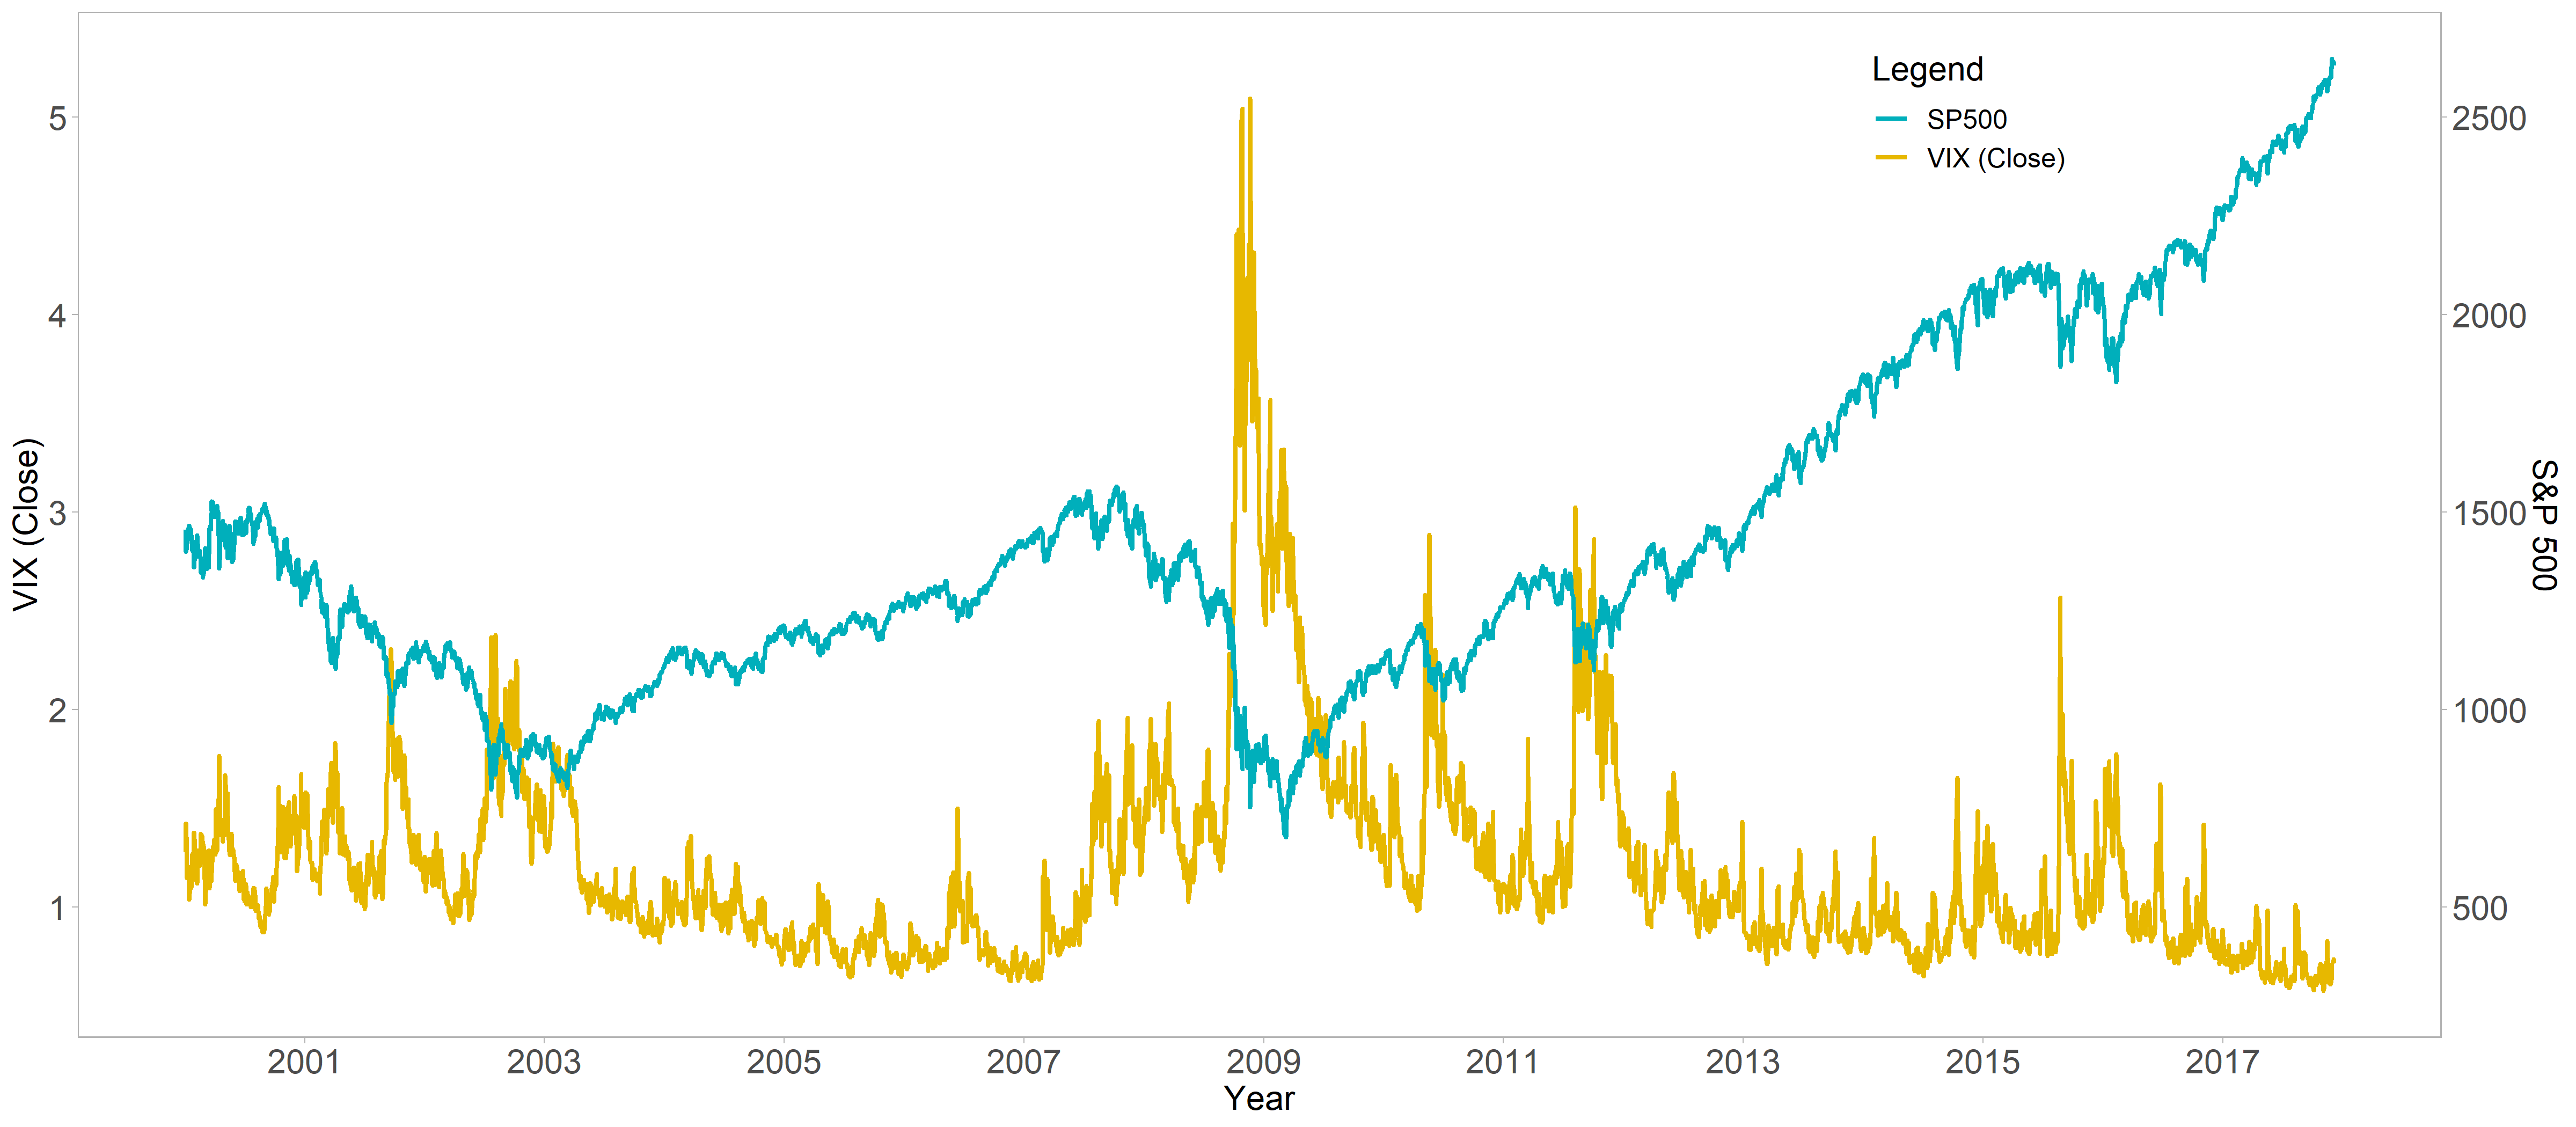
\includegraphics[scale = 0.33]{graphics/SPandViX.png}
	\end{figure}
\end{frame}


\section{Method}

\begin{frame}
\frametitle{}
	\begin{itemize}
	\item Regression of realized volatility on historic volatility
	\end{itemize}
\end{frame}


\section{Results so far}

\begin{frame}
\frametitle{}
	\begin{itemize}
	\item
	\end{itemize}
\end{frame}


\section{Possible Problems coming up}

\begin{frame}
\frametitle{Questions currently to solve}
	\begin{itemize}
	\item Having gathered all this information about volatility measurement, what is the most accurate way to set up my regression?
	
	\end{itemize}
\end{frame}

\section*{Sources}
\begin{frame}
\printbibliography
\end{frame}

\section{Appendix}
\begin{frame}

\end{frame}



\end{document}
